\section{Polarimetría}

\subsection{Ecuación de radar}

\begin{frame}{\secname : \subsecname}
    \begin{block}{Definición}
      \begin{equation}
        P_r \pause \sim \frac{ P_t \pause G_t \pause G_r \pause \lambda^2 \pause \sigma}{\pause R^4}
      \end{equation}
    \end{block}
\end{frame}
%--- Next Frame ---%

\begin{frame}{\secname : \subsecname}
    \begin{block}{Definición}
      \begin{equation}
        P_r = \frac{ P_t  G_t  G_r  \lambda^2  \sigma}{ (4\pi)^3 \ R^4}
      \end{equation}
      Con $P_r$ y $P_t$ las potencias recibidas y transmitidas, $G_r$ y $G_t$ las ganancias del emisor y receptor, $\lambda$ la longitud de onda, $\sigma$ el coeficiente de backscatter o retrodisperción y $R$ la distancia entre el emisor y el blanco.
    \end{block}
\end{frame}
%--- Next Frame ---%

\begin{frame}{\secname : \subsecname}

  \begin{block}{Definición}
    Definimos el coeficiente de retrodispersión por unidad de área de un radar como
    \begin{equation}
      \sigma^0 = \frac{\sigma}{A}
    \end{equation}
    donde $\sigma$ es el coeficiente de retrodispersión y $A$ el área del píxel.
  \end{block}
  \pause
    \begin{block}{Definición}
      Es común expresar el coeficiente de retrodispersión por unidad de área como
      \begin{equation}
        \sigma^0 [dB] = 10\log_{10}(\sigma^0).
      \end{equation}
    \end{block}
%\pause
    %\begin{block}{Definición}
    %  Es común expresar el coeficiente de retrodispersión de un radar en decibels cómo
    %  \begin{equation}
    %    \sigma [dB] = 10\log_{10}(\sigma)
    %  \end{equation}
    %  donde $\sigma$ es el coeficiente de retrodispersión.
    %\end{block}
\end{frame}
%--- Next Frame ---%

\subsection{Polarización}

\begin{frame}{\secname : \subsecname}
  \begin{figure}
    \centering
    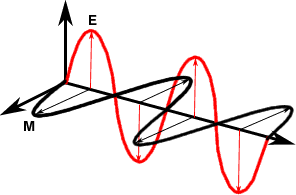
\includegraphics[width=0.5\textwidth]{fig:onda.png}
    \caption{Una onda electromagnética es una oscilación en el campo electromagnético, puede estar orientada en distintas direcciones, llamadas estado de polarización.}
    \label{}
  \end{figure}
\end{frame}
%--- Next Frame ---%

\begin{frame}{\secname : \subsecname}
  \begin{figure}
    \centering
    \movie[width = 0.8\textwidth,loop,autostart]{\centering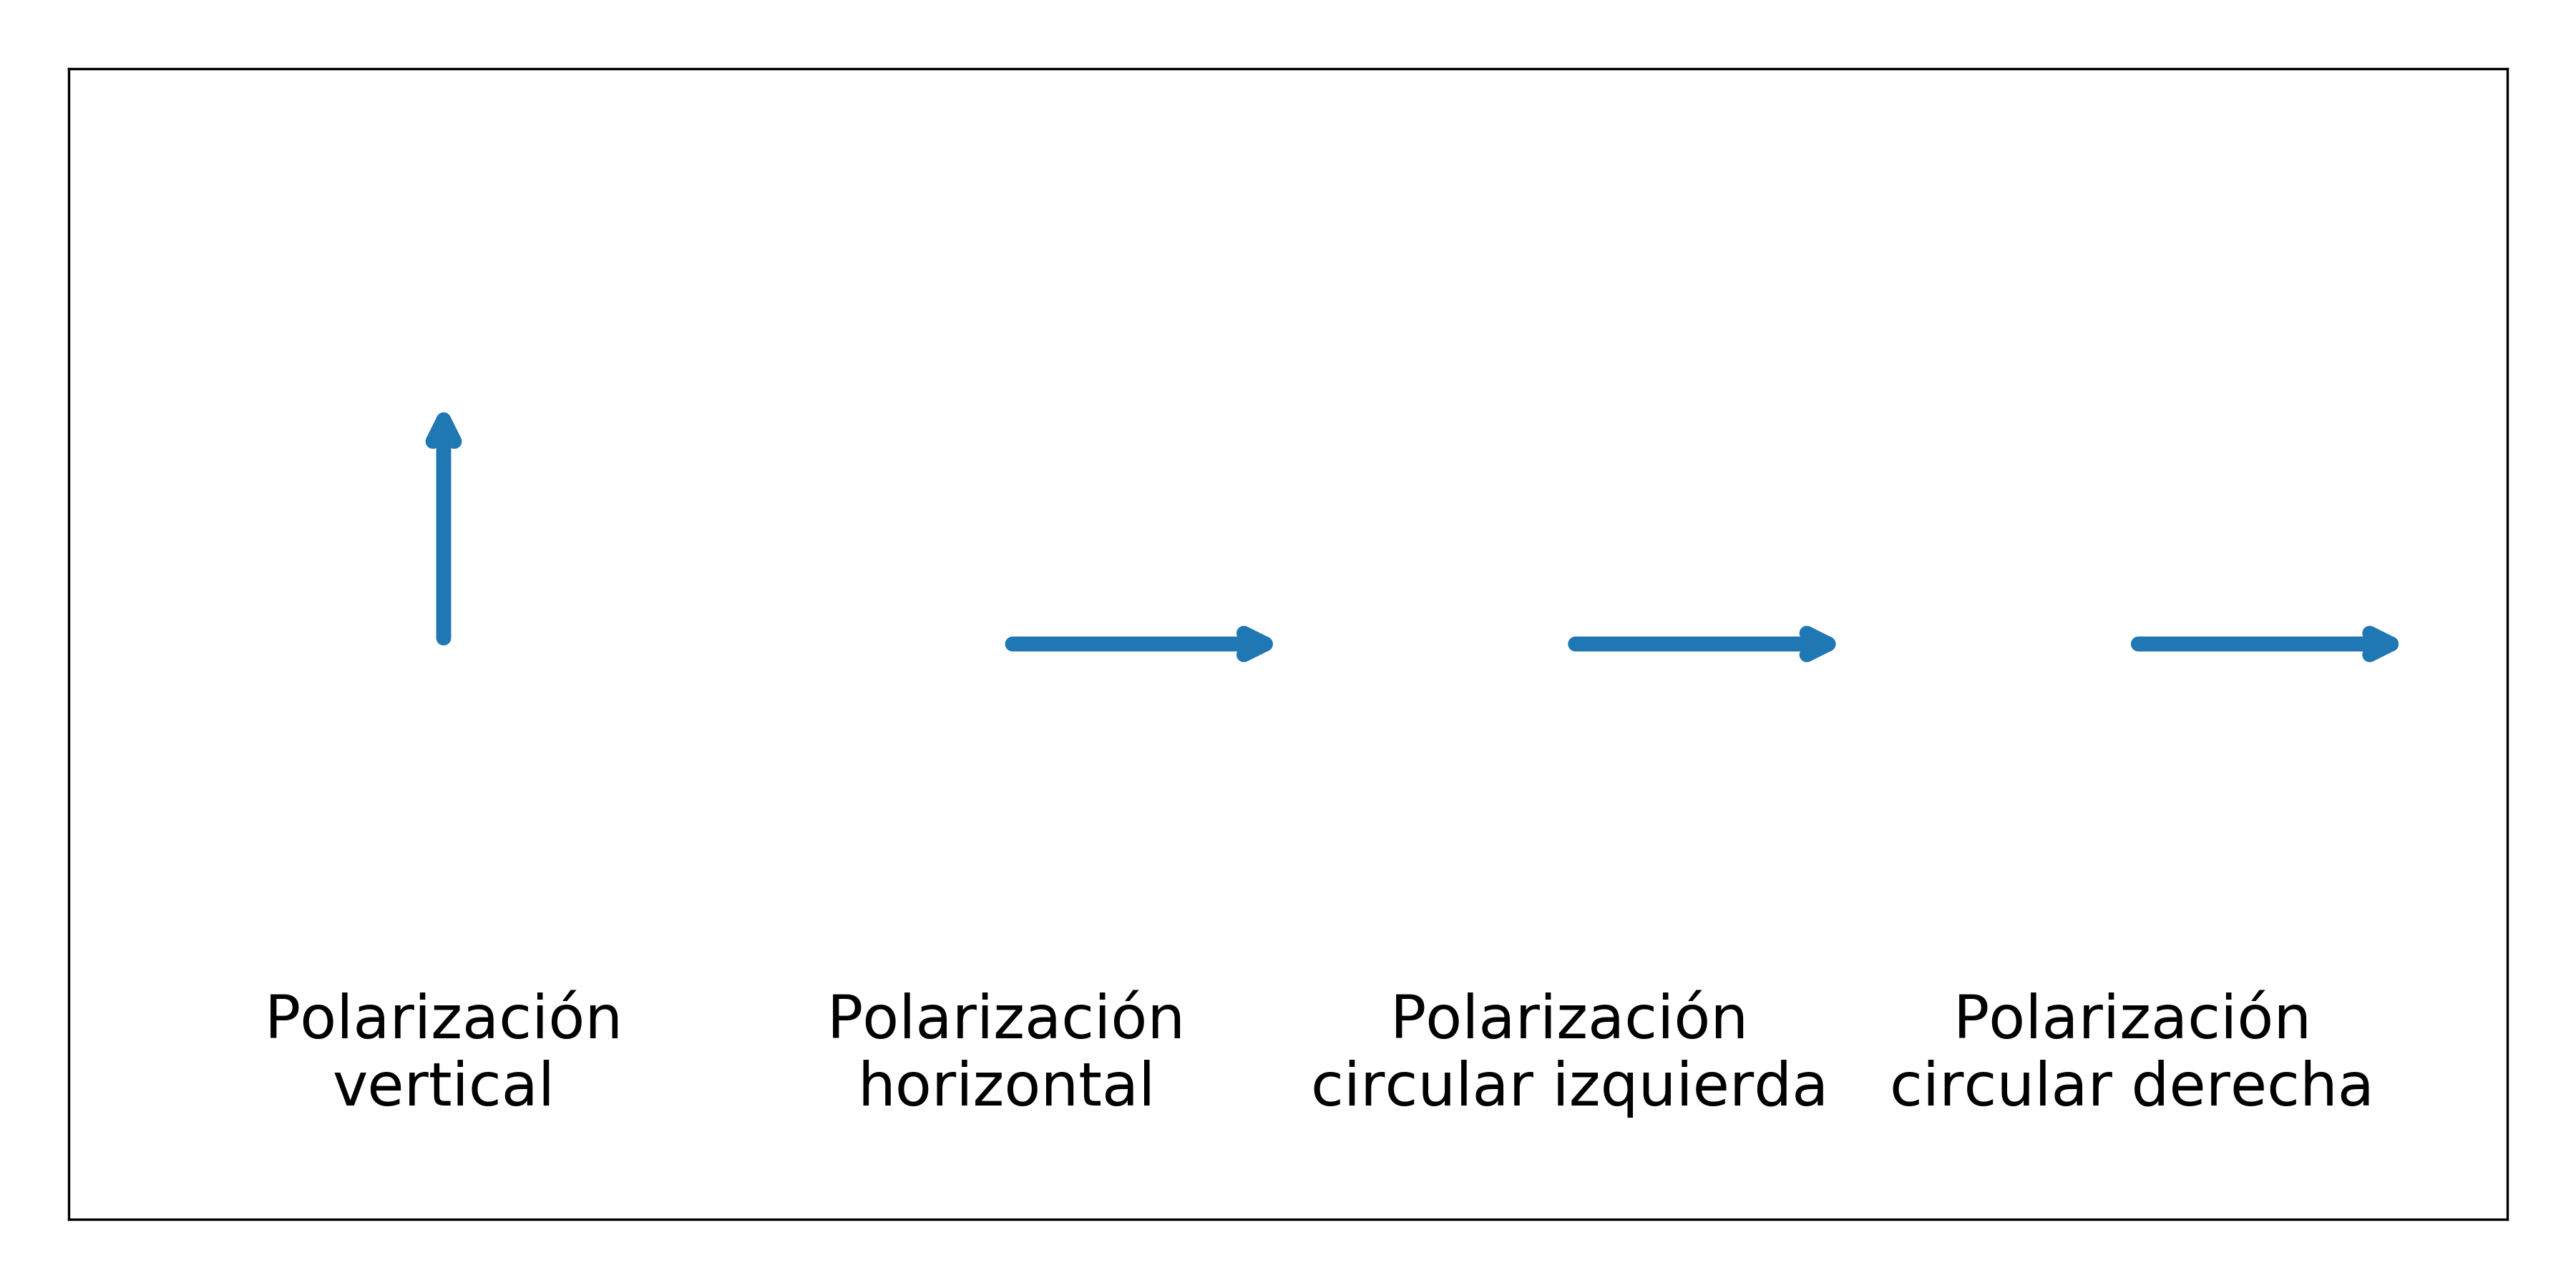
\includegraphics[width=0.8\textwidth]{fig:polarizado.png}}{./figs/fig:polarizado.mp4}
    \caption{Entre los estados de polarización más típicos se pueden destacar la polarización lineal y la circular.}
    \label{}
  \end{figure}
\end{frame}
%--- Next Frame ---%



\begin{frame}{\secname : \subsecname}
  \begin{figure}
    \centering
    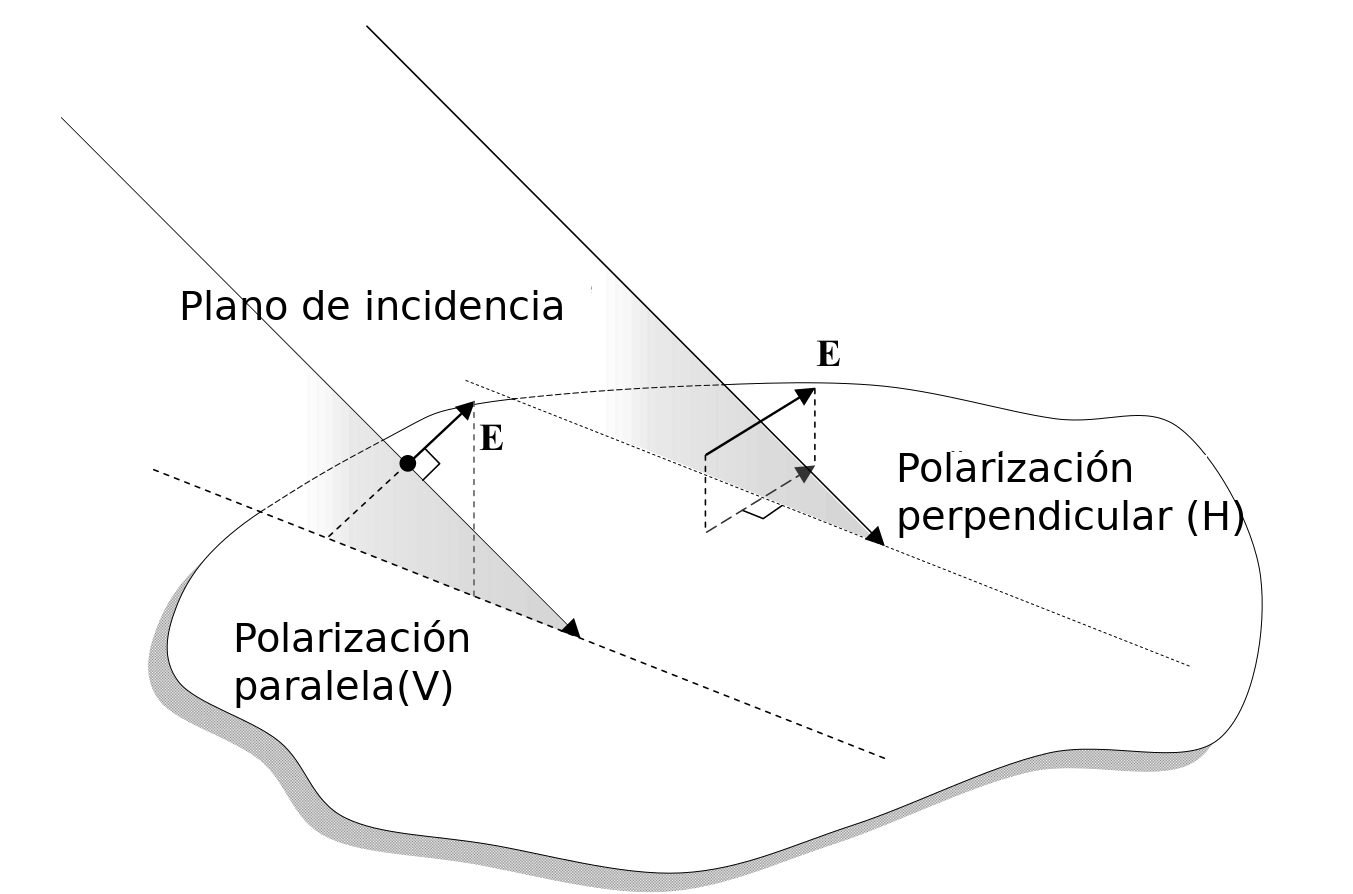
\includegraphics[width=0.55\textwidth]{fig:polarizacion.png}
    \caption{Algunos SAR pueden emitir y recibir tanto en H (Horizontal) -perpendicular al plano de incidencia-, como en V (Vertical) -paralela al plano de incidencia-. Combinándolas entre transmisión y recepción se obtienen 4 combinaciones polarimétricas: {\bf HH, HV, VH, y VV}.}
    \label{}
  \end{figure}
\end{frame}
%--- Next Frame ---%

\begin{frame}{\secname : \subsecname}
  \begin{figure}
    \centering
    \subfloat[Polarización HH]{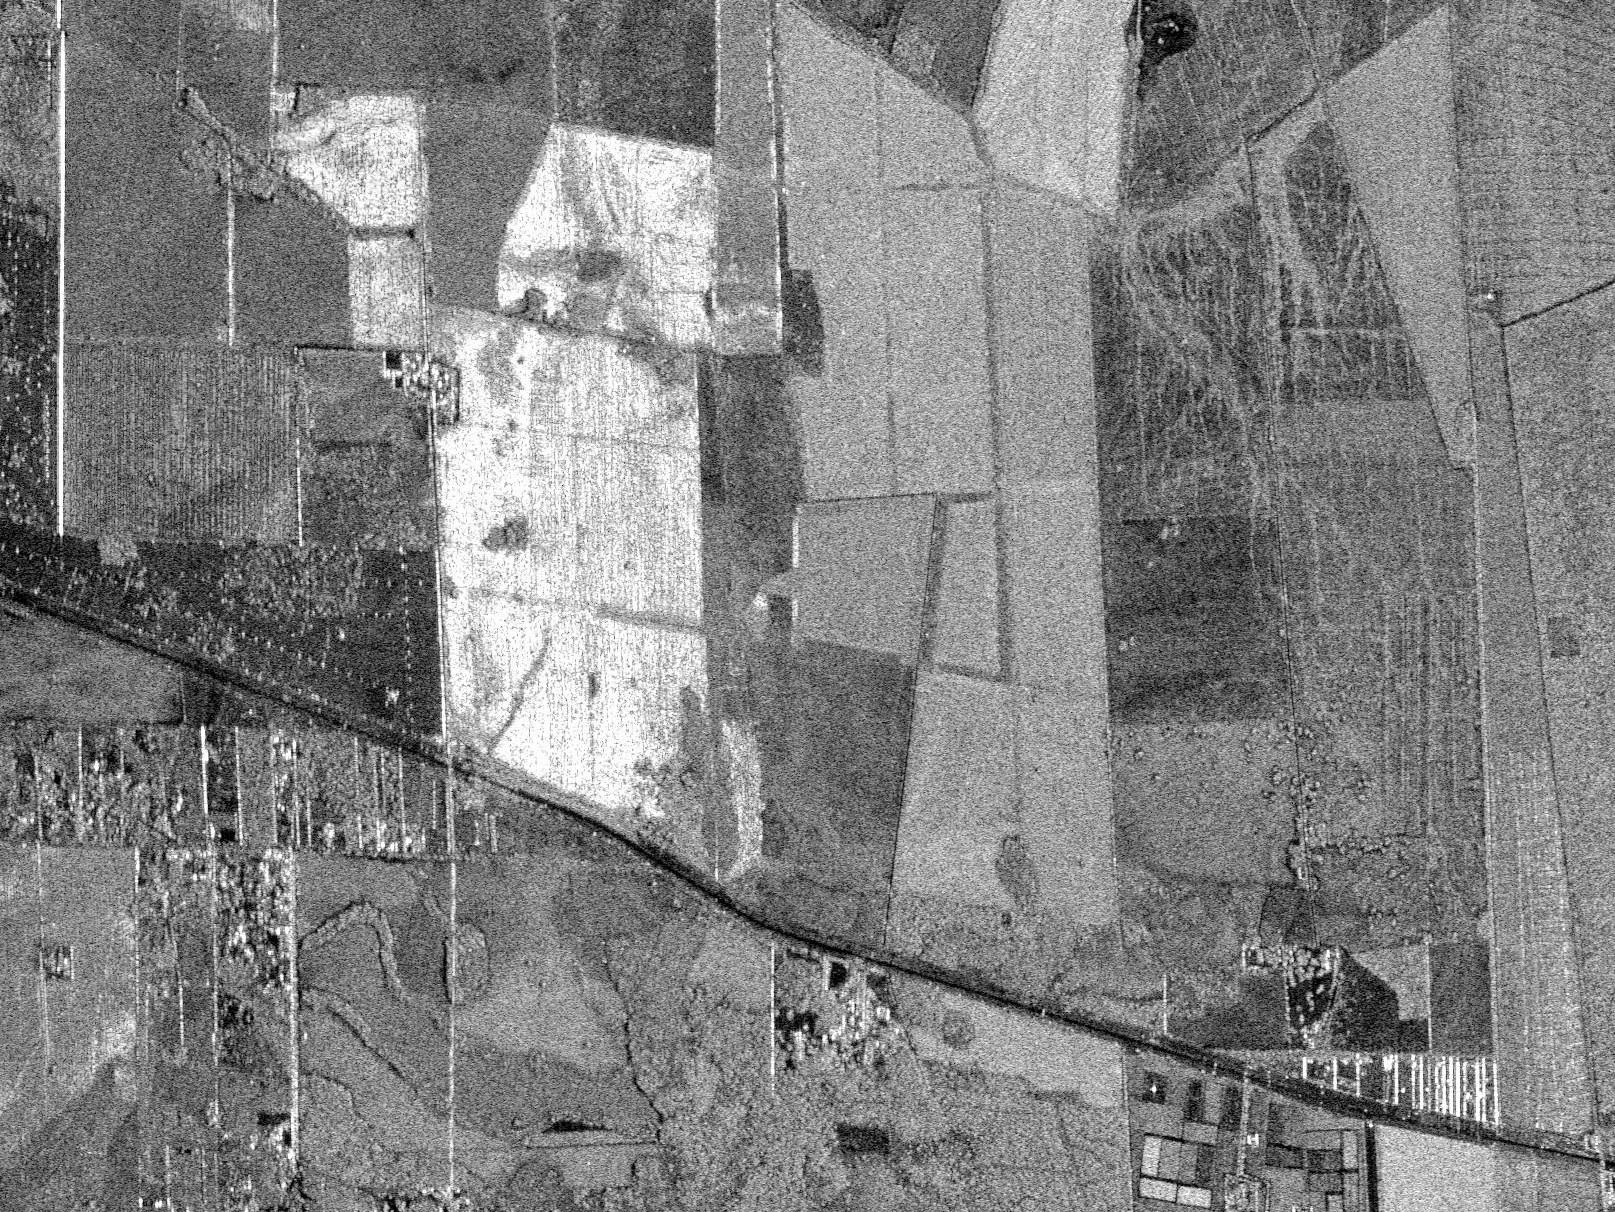
\includegraphics[width=0.25\textwidth]{fig:HH.jpg}}\hspace{1cm}
    \subfloat[Polarización HV]{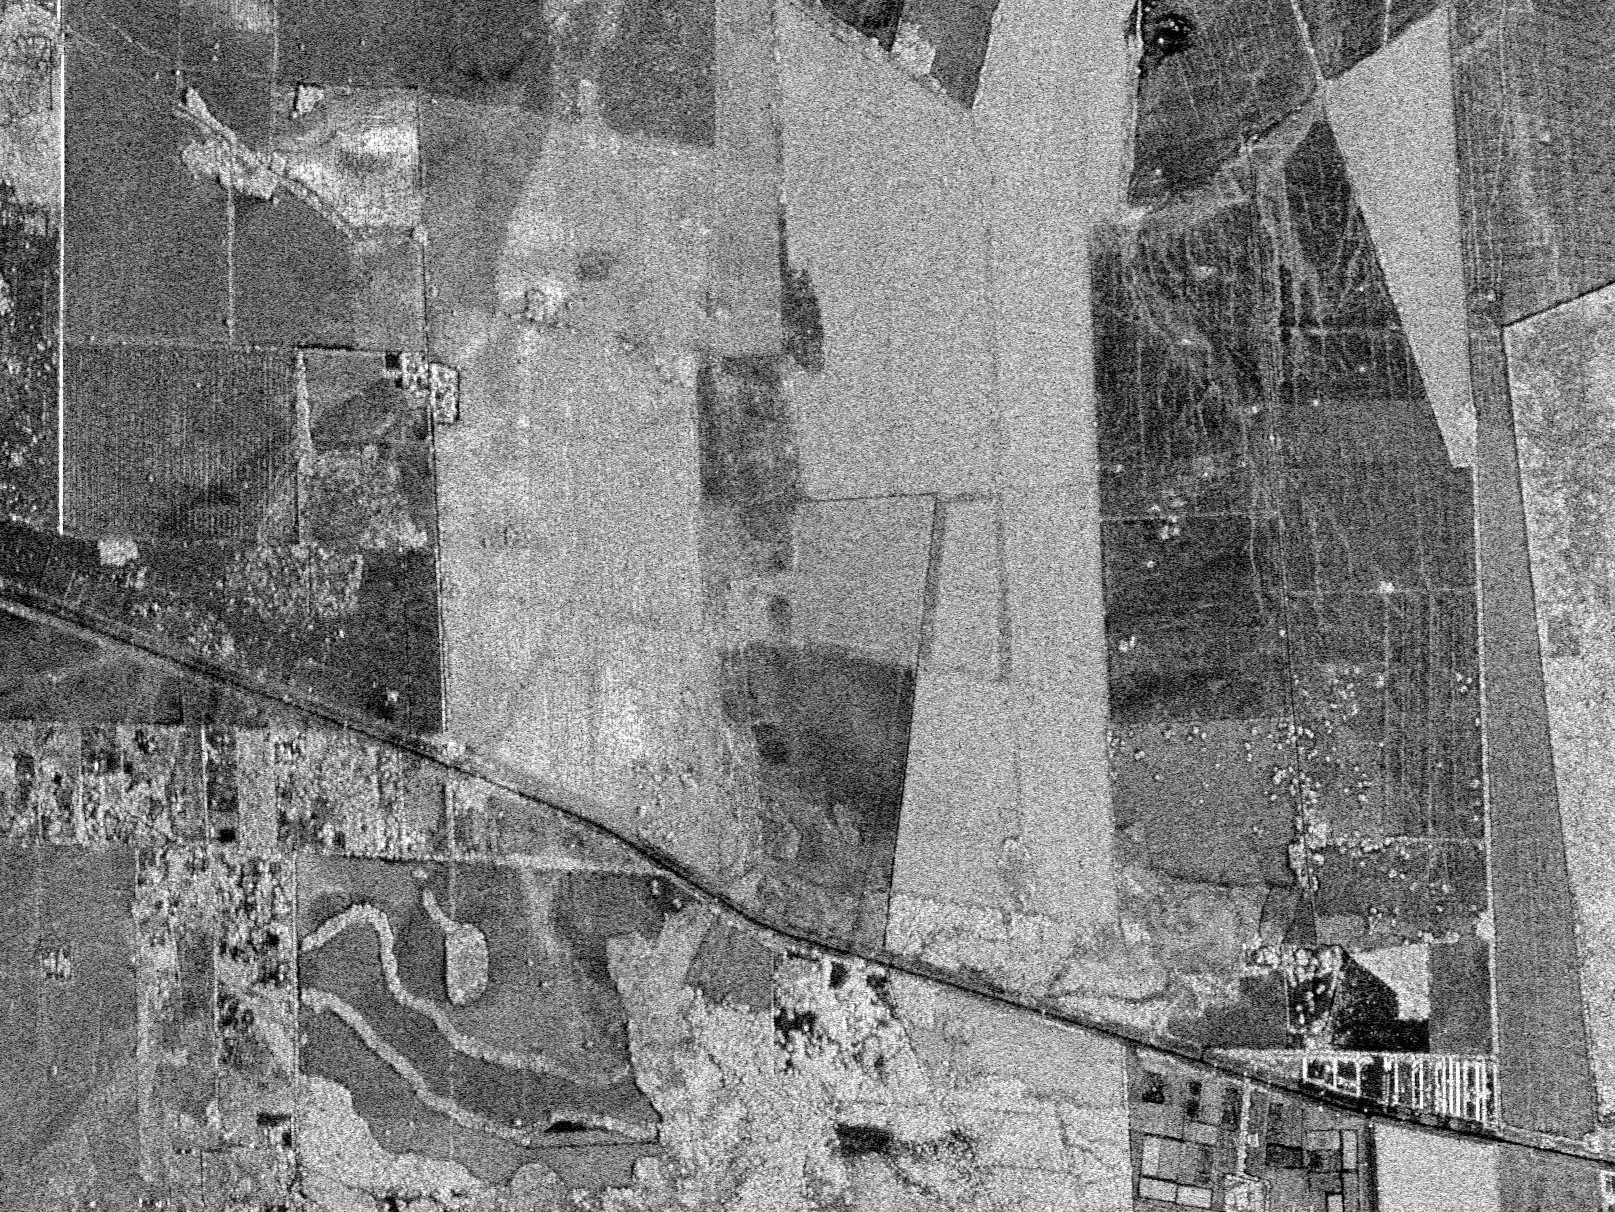
\includegraphics[width=0.25\textwidth]{fig:HV.jpg}}
    \\
    \subfloat[Polarización VH]{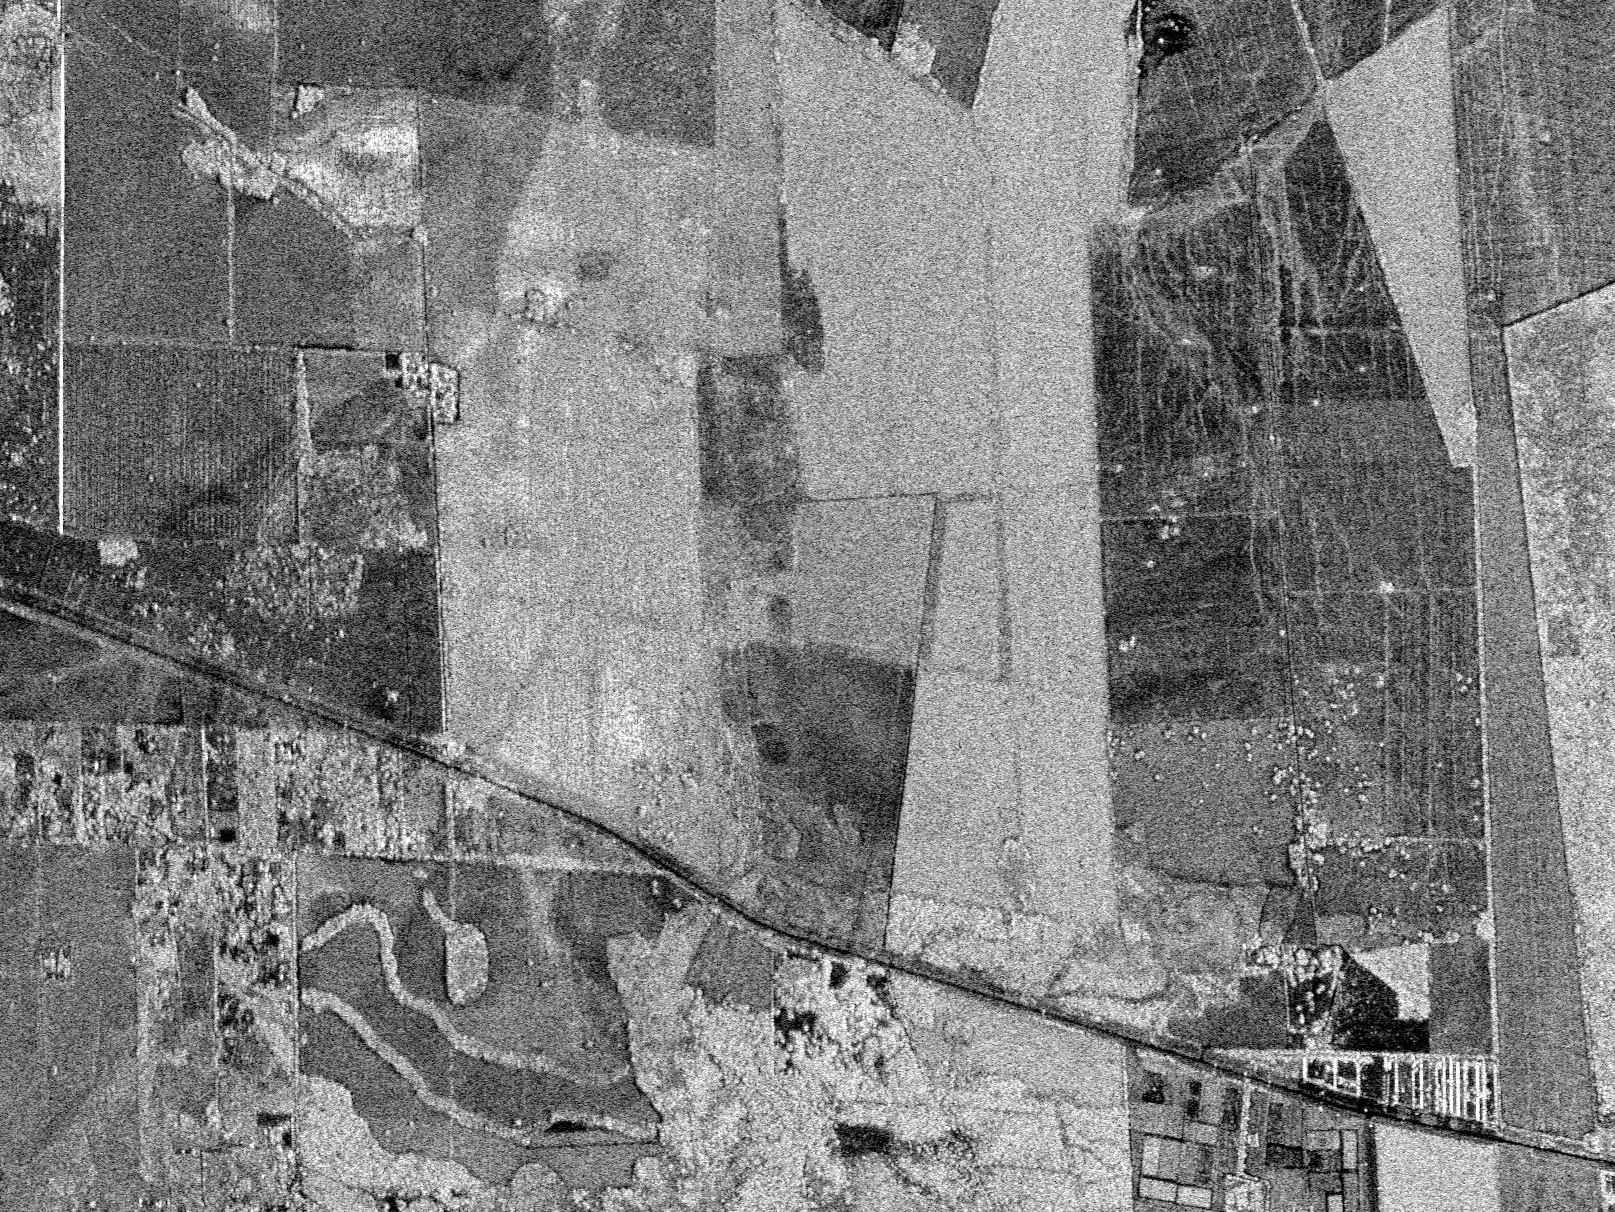
\includegraphics[width=0.25\textwidth]{fig:VH.jpg}}\hspace{1cm}
    \subfloat[Polarización VV]{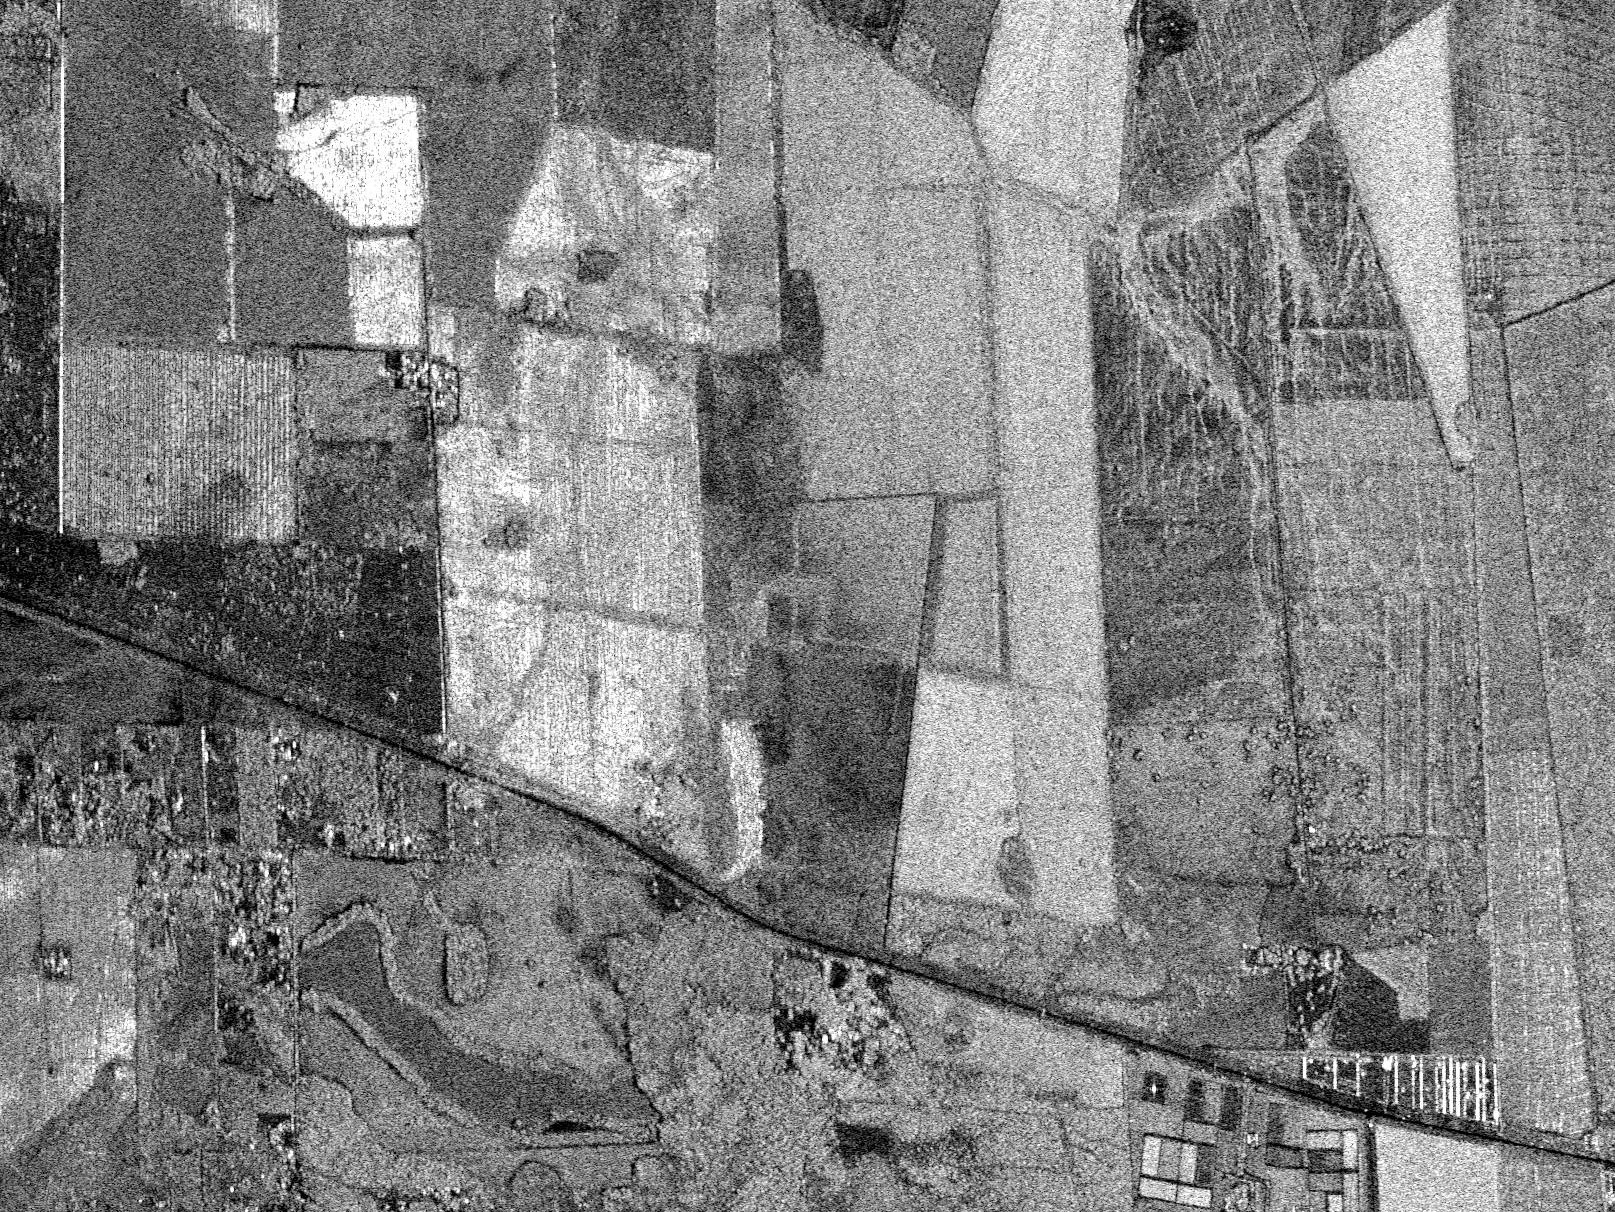
\includegraphics[width=0.25\textwidth]{fig:VV.jpg}}
    \caption{Distintas polarizaciones para una misma región.}
  \end{figure}
\end{frame}
%--- Next Frame ---%

%\begin{frame}{\secname : \subsecname}
%  En este caso la representación del coeficiente de backscatter es matricial
%  \begin{columns}
%    \begin{column}{0.5\textwidth}
%     \begin{block}{Matriz de scattering}
%      \begin{equation}
%        S=
%  \begin{bmatrix}
%    S_{HH} & S_{HV} \\
%    S_{VH} & S_{VV}
%  \end{bmatrix}
%      \end{equation}
%     \end{block}
%    \end{column}
%    \begin{column}{0.5\textwidth}  %%<--- here
%      \begin{block}{Matriz de backscatter}
%        \begin{equation}
%          \sigma_0= \frac{1}{A}
%  \begin{bmatrix}
%    |S_{HH}|^2 & |S_{HV}|^2 \\
%    |S_{VH}|^2 & |S_{VV}|^2
%  \end{bmatrix}
%        \end{equation}
%        con $A$ el area del píxel.
%      \end{block}
%    \end{column}
%    \end{columns}
%\end{frame}
%--- Next Frame ---%

\subsection{Descoposición de Pauli}

\begin{frame}{\secname : \subsecname}
     \begin{block}{Descomposición de Pauli}
      \begin{equation}
        R = \left(\frac{HH-VV}{\sqrt{2}}\right)^2
      \end{equation}
      \begin{equation}
        G = \left(\sqrt{2}HV\right)^2
      \end{equation}
      \begin{equation}
        B = \left(\frac{HH+VV}{\sqrt{2}}\right)^2
      \end{equation}
     \end{block}
    La descomposición de Pauli es una manera de visualizar los distintos mecanismo de scattering presentes: azul -especular-, verde -en volumen- y rojo -doble rebote-.
\end{frame}
%--- Next Frame ---%

\begin{frame}{\secname : \subsecname}
  \begin{figure}
    \centering
    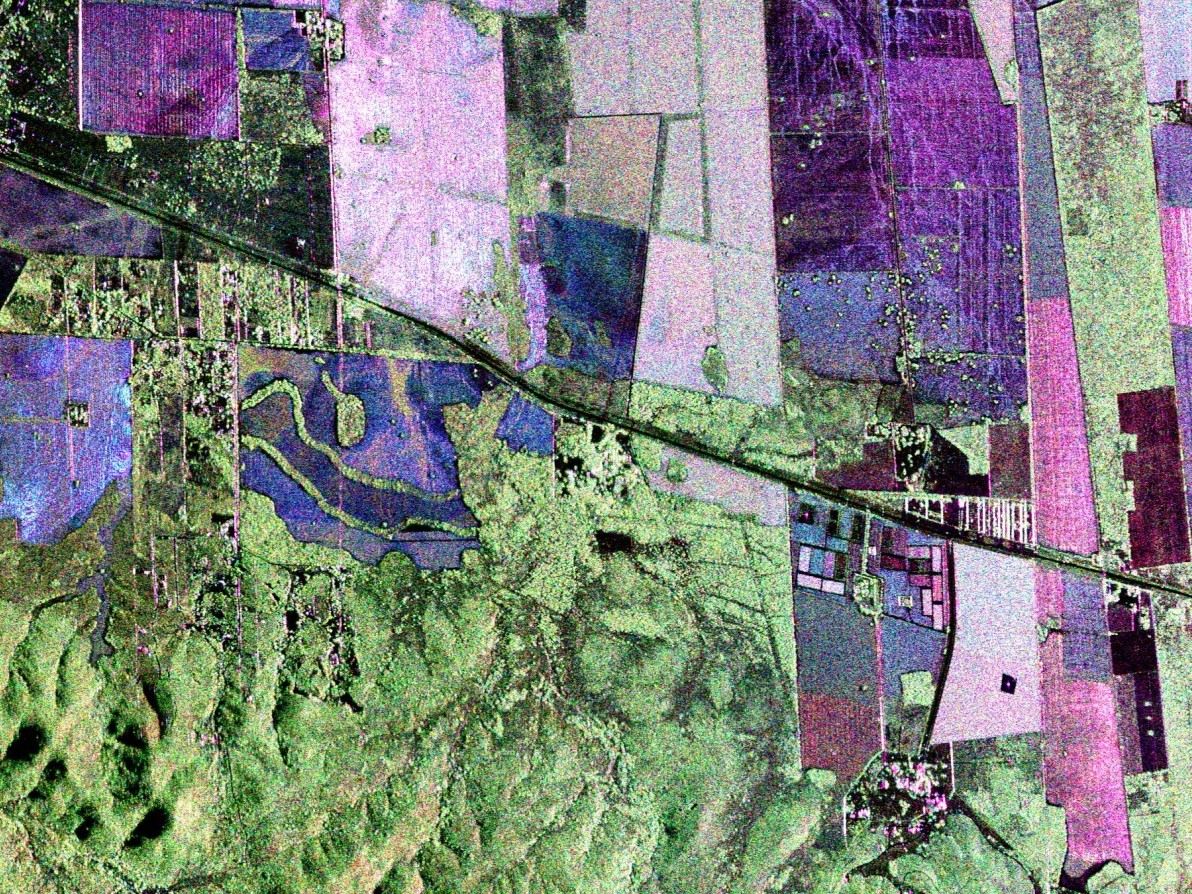
\includegraphics[width=0.5\textwidth]{fig:rgbpauli}
    \caption{Descomposición de Pauli en combinación RGB.}
    \label{}
  \end{figure}
\end{frame}
%--- Next Frame ---%

\begin{frame}{\secname : \subsecname}
Muchas gracias.
\end{frame}
%--- Next Frame ---%
